\documentclass{exam}
\usepackage[utf8]{inputenc}
\usepackage{lmodern}
\usepackage{microtype}

% \usepackage[parfill]{parskip}
\usepackage[dvipsnames]{xcolor}
\usepackage{amsmath}
\usepackage{amsfonts}
\usepackage{amsthm}
\usepackage{siunitx}
\DeclareSIUnit\year{yr}
\DeclareSIUnit\foot{ft}
\DeclareSIUnit\litre{\liter}

\usepackage{skull}

\usepackage{pgfplots}
\usepgfplotslibrary{polar}
\pgfplotsset{compat=1.11}
\usepgfplotslibrary{statistics}
\usepackage{graphicx}
\usepackage{sidecap}
\sidecaptionvpos{figure}{c}
\usepackage{float}
\usepackage{gensymb}
\usepackage{tkz-euclide}
\usetkzobj{all}
\usepackage{commath}
\usepackage{hyperref}
\usepackage{enumitem}
\usepackage{wasysym}
\usepackage{multicol}
\usepackage{mathtools}
\usepackage{tcolorbox}
\usepackage{tabularx}
\usepackage[version=4]{mhchem}
\usepackage{changepage}
\usepackage{listings}
\lstset{basicstyle=\ttfamily\linespread{0.8}\small}

\renewcommand*{\thefootnote}{\fnsymbol{footnote}}

\newtheorem*{thm}{Theorem}
\newtheorem*{iden}{Identity}
\newtheorem*{lemma}{Lemma}
\newtheorem{obs}{Observation}
\theoremstyle{definition}
\newtheorem*{defn}{Definition}
\newtheorem*{ex}{Example}
\newtheorem{con}{Construction}
\newtheorem*{alg}{Algorithm}

\newtheoremstyle{break}
  {\topsep}{\topsep}%
  {\itshape}{}%
  {\bfseries}{}%
  {\newline}{}%
\theoremstyle{break}
\newtheorem*{bthm}{Theorem}

% russian integral
\usepackage{scalerel}
\DeclareMathOperator*{\rint}{\scalerel*{\rotatebox{17}{$\!\int\!$}}{\int}}

% \DeclareMathOperator*{\rint}{\int}

\pgfplotsset{vasymptote/.style={
    before end axis/.append code={
        \draw[densely dashed] ({rel axis cs:0,0} -| {axis cs:#1,0})
        -- ({rel axis cs:0,1} -| {axis cs:#1,0});
    }
}}

% \pointsinrightmargin
\boxedpoints
\pointname{}

\newcommand{\questioA}{\question[\texttt{\textbf{\color{Cerulean} A}}]}
\newcommand{\questioM}{\question[\texttt{\textbf{\color{PineGreen} M}}]}
\newcommand{\questioE}{\question[\texttt{\textbf{\color{WildStrawberry} E}}]}
\newcommand{\questioS}{\question[\texttt{\textbf{\color{Goldenrod} S}}]}
\newcommand{\questioO}{\question[\texttt{\textbf{\color{BurntOrange} O}}]}

\newcommand{\parA}{\part[\texttt{\textbf{\color{Cerulean} A}}]}
\newcommand{\parM}{\part[\texttt{\textbf{\color{PineGreen} M}}]}
\newcommand{\parE}{\part[\texttt{\textbf{\color{WildStrawberry} E}}]}
\newcommand{\parS}{\part[\texttt{\textbf{\color{Goldenrod} S}}]}
\newcommand{\parO}{\part[\texttt{\textbf{\color{BurntOrange} O}}]}

\newcommand{\subparA}{\subpart[\texttt{\textbf{\color{Cerulean} A}}]}
\newcommand{\subparM}{\subpart[\texttt{\textbf{\color{PineGreen} M}}]}
\newcommand{\subparE}{\subpart[\texttt{\textbf{\color{WildStrawberry} E}}]}
\newcommand{\subparS}{\subpart[\texttt{\textbf{\color{Goldenrod} S}}]}
\newcommand{\subparO}{\subpart[\texttt{\textbf{\color{BurntOrange} O}}]}

\newcommand{\mainHeader}[2]{\section*{NCEA Level 2 Mathematics\\#1. #2}}
\newcommand{\mainHeaderHw}[2]{\section*{NCEA Level 2 Mathematics (Homework)\\#1. #2}}
\newcommand{\seealso}[1]{\begin{center}\emph{See also #1.}\end{center}}
\newcommand{\drills}[1]{\begin{center}\emph{Drill problems: #1.}\end{center}}
\newcommand{\basedon}[1]{\begin{center}\emph{Notes largely based on #1.}\end{center}}

\begin{document}

\mainHeaderIntg{26}{More Interesting Problems}
These problems do not just concern integration.
\subsection*{Questions}
\begin{questions}
  \questioE Find the equation of the line through the point $ (3,5) $ which cuts off the least area from the first quadrant.
  \questioE The area of a square is increasing at a constant rate of $ k~\si{\metre\squared} $ per second. A tetrahedron (equilateral triangular pyramid),
            has a side length that is the same as that of the square at each instant. The initial volume of the tetrahedron was \SI{1}{\metre\cubed}.
            In terms of $ k $, what is the volume of the tetrahedron three seconds after that?
  \questioS Scholarship 2017: The hyperbolic functions $ \sinh x $ and $ \cosh x $ are defined as follows:
            \begin{gather*}
              \sinh x = \frac{1}{2} (e^x - e^{-x})\\
              \cosh x = \frac{1}{2} (e^x + e^{-x}).
            \end{gather*}
            Show that $ \od{}{x} \sinh^{-1} x = \frac{1}{\sqrt{x^2 + 1}} $.
  \questioS Consider the tetrahedron inscribed inside a cube, as in the figure.
            \begin{center}
              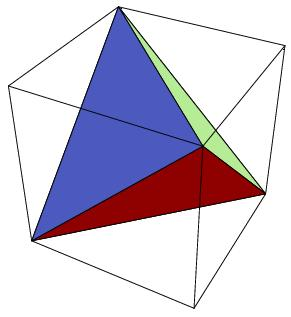
\includegraphics[width=0.2\textwidth]{tetrahedron}
            \end{center}
            The volume $ V $ of the cube at any instant $ t $ is increasing at a rate proportional to the value of $ V $ at that instant. The
            initial volume of the cube at $ t = 0 $ was 8 cubic units. What is the volume of the tetrahedron at time $ t = 20 $?
  \questioS If $ x \sin \pi x = \rint^{x^2}_0 f(t) \dif{t} $, where $ f $ is continuous, find $ f(4) $. [\textit{Hint: you need not perform any integration.}]
  \questioS If $ f $ and $ g $ are differentiable functions with $ f(0) = g(0) = 0 $ and $ g'(0) \neq 0 $, show that
            \begin{displaymath}
              \lim_{x \to 0} \frac{f(x)}{g(x)} = \frac{f'(0)}{g'(0)}.
            \end{displaymath}
            Hence, or otherwise, evaluate
            \begin{displaymath}
              \lim_{x \to 0} \frac{\sin(a + 2x) - 2\sin(a + x) + \sin a}{x^2}.
            \end{displaymath}
  \question
    \begin{parts}
      \parS Consider the differential equation
            \begin{displaymath}
              \od[2]{\Phi}{t} + 5\od{\Phi}{t} + 6\Phi(t) = 0.
            \end{displaymath}
            Let $ f $ and $ g $ be the functions defined by $ f(x) = e^{-2x} $ and $ g(x) = e^{-3x} $.
            \begin{subparts}
              \subpart Show that all linear combinations of $ f $ and $ g $ are solutions to the differential equation.
              \subpart Find the (unique) solution passing through $ (0,1) $ and $ (1,1) $.
            \end{subparts}
      \parO More generally, consider the differential equation $ a\od[2]{y}{x} + b\od{y}{x} + cy = 0 $. Let
            the zeroes of the quadratic polynomial $ p(D) = aD^2 + bD + c $ be $ \alpha $ and $ \beta $. Show
            that all the linear combinations of $ e^{\alpha x} $ and $ e^{\beta x} $ are solutions to the differential
            equation.
    \end{parts}
  \questioS Compute the following definite integral. [\textit{Hint: begin with a substitution.}]
            \begin{displaymath}
              \rint_0^{\pi/6} \sqrt{\tan \theta} \dif{\theta}
            \end{displaymath}
  \question
    \begin{parts}
      \parE Consider the two functions $ p(x) = 3x^5 - 5x^3 + 2x $ and $ q(x) = 3x^5 $. Show that their ratio approaches
            1 as $ x \to \infty $.
      \parS Let $ p(x) $ and $ q(x) \neq 0 $ be polynomials. Recall that the degree of a polynomial is the highest $ n $ such that $ x^n $
            has a non-zero coefficient. Compute the limit
            \begin{displaymath}
              \lim_{x \to \infty} \frac{p(x)}{q(x)}
            \end{displaymath}
            if:
        \begin{subparts}
          \subpart the degree of $ p(x) $ is less than that of $ q(x) $.
          \subpart the degree of $ p(x) $ is greater than that of $ q(x) $.
        \end{subparts}
    \end{parts}
  \questioS A definite integral calculates the between a curve and straight line, the $ x$-axis. In a similar way, it is possible
            to use integration to calculate the area above a curved line and below a surface $ z = f(x,y) $, like that in the figure.
            \begin{center}
              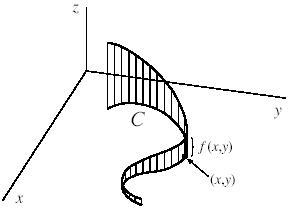
\includegraphics[width=0.3\textwidth]{contourintegral}
            \end{center}
            If the curve $ C $ is defined parametrically, that is $ C(t) = (x(t), y(t)) $, then the integral along the line can be
            calculated with the formula
            \begin{displaymath}
              \rint_a^b f(x(t), y(t)) \sqrt{\left(\dod{x}{t}\right)^2 + \left(\dod{y}{t}\right)^2} \dif{t}.
            \end{displaymath}
            Compute the line integral of the function $ f(x,y) = 2 + x^2 y $ around the upper half of the unit circle.
  \questioS The \textbf{sine integral} function is defined by
            \begin{displaymath}
              \mathrm{Si}(x) =
              \begin{cases}
                \rint^x_0 \frac{\sin t}{t} \dif{t}, &\text{for $ x \neq 0 $;}\\
                1, &\text{for $ x = 0 $.}
              \end{cases}
            \end{displaymath}
    \begin{parts}
      \part Recall that $ \rint^b_a f'(t) \dif{t} = f(b) - f(a) $. Use this to show that $ \od{}{x} \rint^x_0 f'(t) \dif{t} = f'(x) $.
      \part Find the $ x$-coordinate of the first local maximum of $ \textrm{Si} $ to the right of the origin. Carefully prove that you have
            found a maximum.
      \part Use the result in (a) to find an expression for the integral
            \begin{displaymath}
              \od{}{x} \rint^{h(x)}_{g(x)} f(t) \dif{t},
            \end{displaymath}
            where $ f $ is continuous and $ g $ and $ h $ are differentiable.
    \end{parts}
  \questioE Minimise the function $ f(x) = b\log_b N $ with respect to $ b $, and show that the result is independent of the
            constant $ N $.\footnote{~Dudley, \textit{Mathematical Cranks}, p.52.}
  \questioS We can calculate \textbf{improper integrals} (those where the bounds are infinite) as follows:
            \begin{displaymath}
              \rint^{\infty}_a f(x) \dif{x} = \lim_{b \to \infty} \rint^b_a f(x) \dif{x}.
            \end{displaymath}
            Decide whether each of the integrals given below exists. If so, calculate its value; if not, explain why.
    \begin{multicols}{3}
    \begin{parts}
      \part $ \displaystyle \rint^{\infty}_1 \frac{1}{x} \dif{x} $
      \part $ \displaystyle \rint^{\infty}_1 \frac{1}{x^2} \dif{x} $
      \part $ \displaystyle \rint^{\infty}_1 \sin x \dif{x} $
    \end{parts}
    \end{multicols}
  \question
    \begin{parts}
      \parS Show that $ F(x) = \tan^{-1} x $ is an anti-derivative of $ f(x) = \frac{1}{1 + x^2} $ in the following ways:
        \begin{subparts}
          \subpart Differentiate $ F(x) $ and simplify to give $ f(x) $.
          \subpart Use the substitution $ x = \tan \theta $ to integrate $ f(x) $ and simplify to give $ F(x) $.
        \end{subparts}
      \parO Recall that $ 22/7 $ is often given as a rough approximation to $ \pi $. Consider the integral
            \begin{displaymath}
              I = \rint^1_0 \frac{x^4(1-x)^4}{1 + x^2} \dif{x},
            \end{displaymath}
            and hence show that $ 22/7 > \pi $.\footnote{~Nahin, \textit{Inside Interesting Integrals}, pp.23-4.}
    \end{parts}
  \questioS Consider the operator $ \mathcal{L} $ defined by
            \begin{displaymath}
              \mathcal{L} f(x) = \od{}{x} \ln\left[f\left(e^x\right)\right].
            \end{displaymath}
    \begin{parts}
      \part Show that $ \mathcal{L} x^n = n $ and that $ \mathcal{L} [u(x)]^n = n \mathcal{L} u(x) $.
      \part Find an expression for $ \mathcal{L} [u(x) v(x)] $ and $ \mathcal{L} [u(x)/v(x)] $.
      \part Find an expression for $ \mathcal{L} [u(x) + v(x)] $.
      \part For which $ y $ is $ \mathcal{L} y = y $?
    \end{parts}
  \questioS Compute the following indefinite integrals:
    \begin{parts}
      \part $ \displaystyle \rint \frac{\sin \frac{1}{x}}{x^2} \dif{x} $
      \part $ \displaystyle \rint \frac{\ln x \cos x - \frac{\sin x}{x}}{(\ln x)^2} \dif{x} $
    \end{parts}
  \clearpage
  \questioO A while ago (when we talked about the product and quotient rules), I claimed that the radius of the circle best approximating a continuous
            curve around a point $ (x,y) $ is given by
            \begin{displaymath}
              \textrm{radius of curvature} = \frac{\left[1 +  \left(\od{y}{x}\right)^2 \right]^{\frac{3}{2}}}{\abs{\od[2]{y}{x}}}.
            \end{displaymath}
            Let us attempt to prove this.
    \begin{parts}
      \part Let $ f $ be a continuous function at $ x $ such that the second derivative of $ f $ at $ x $ exists. By recalling our work on approximations,
            explain why knowing up to the second derivative of $ f $ should be enough to find the `best circular approximation' of $ f $ at $ (x, f(x)) $.
      \part Consider the circle of radius $ r $ centred at $ (x_0, y_0) $. Suppose that this circle passes through the point $ (x_1, y_1) $;
            suppose further that the first derivative of the $ y$-ordinate of the circle with respect to the $ x$-ordinate is $ m $, and that
            the second derivative is $ c $. Write down expressions for $ r $, $ x_0 $, and $ y_0 $ in terms of $ x_1 $, $ y_1 $, $ m $, and $ c $.
      \part Use part (b) to write down the radius of the unique circle passing through $ (x, f(x)) $ with matching first and second derivatives to $ f $.
    \end{parts}
\end{questions}

\end{document}
